\documentclass[11.5pt]{sig-alternate} % sets document style to sig-alternate
% packages
% typesetting
%\usepackage{dirtytalk} % typset quotations easier (\say{stuff})
\usepackage{hanging} % hanging paragraphs
\usepackage[defaultlines=3,all]{nowidow} % avoid widows
\usepackage[pdfpagelabels=false]{hyperref} % produce hypertext links, includes backref and nameref
\usepackage{xurl} % defines url linebreaks, loads url package
\usepackage{microtype}
%\usepackage[super]{nth} % easily create superscript ordinal numbers with \nth{x}
\usepackage{textcomp}
\newcommand{\texttildemid}{\raisebox{0.4ex}{\texttildelow}}
% layout
%\usepackage{enumitem} % control layout of itemize, enumerate, description
\usepackage{fancyhdr} % control page headers and footers
\usepackage{float} % improved interface for floating objects
%\usepackage{multicol} % intermix single and multiple column pages
% language
\usepackage[utf8]{inputenc} % accept different input encodings
\usepackage[english]{babel} % multilanguage support
% misc
\usepackage{graphicx} % builds upon graphics package, \includegraphics
%\usepackage{lastpage} % reference number of pages
%\usepackage{comment} % exclude portions of text (?)
\usepackage{xcolor} % color extensions
\usepackage[backend=biber, style=apa]{biblatex} % sophisticated bibliographies % necessary for HTML to display author info and date on abstract page
\usepackage{csquotes} % advanced quotations, makes biblatex happy
\usepackage{authblk} % support for footnote style author/affiliation
% tables and figures
\usepackage{tabularray}
%\usepackage{array} % extend array and tabular environments
\usepackage{caption} % customize captions in figures and tables (rotating captions, sideways captions, etc)
%\usepackage{cuted} % allow mixing of \onecolumn and \twocolumn on same page
\usepackage{multirow} % create tabular cells spanning multiple rows
%\usepackage{subfigure} % deprecated, support for manipulation of small figures
%\usepackage{tabularx} % extension of tabular with column designator "x", creates paragraph-like column whose width automatically expands
%\usepackage{wrapfig} % allows figures or tables to have text wrapped around them
%\usepackage{booktabs} % better rules
% dummy text
%\usepackage{blindtext} % blind text dummy text
%\usepackage{kantlipsum} % Kant style dummy text
\usepackage{lipsum} %lorem ipsum dummy text
% other helpful packages may be booktabs, longtable, longtabu, microtype

\pagestyle{fancy} % sets pagestyle to fancy for fancy headers and footers

% header and footer
% modern way to set header image
\renewcommand{\headrulewidth}{0pt} % defines thickness of line under header
\renewcommand{\footrulewidth}{0pt} % defines thickness of line above header
\setlength\headheight{80.0pt} % sets height between top margin and header image, effectively moves page contents down
\addtolength{\textheight}{-80.0pt} % seems to affect the lower height. maybe only works properly if footer numbers enabled?
\fancyhf{}
\fancyhead[CE, CO]{
\includegraphics[width=\textwidth]{headerImage.png}}
% footer
%\fancyfoot[LE,LO]{Article Title Here \\ DOI: }% left footer article title and doi
%\fancyfoot[CE,CO]{{}} % center footer empty
%\fancyfoot[RE,RO]{\thepage} % right footer page numbers
%\pagenumbering{arabic} % arabic (1, 2, 3) numbering in footer

\hypersetup{colorlinks=true,urlcolor=blue} % sets link color to blue
\urlstyle{same} % sets url typeface to same as rest of text

% set caption and figure to italics, label bold, left align captions, does not transfer to HTML
\captionsetup{labelfont=bf, font={large, it}, justification=raggedright, singlelinecheck=false}
\renewcommand\theContinuedFloat{\alph{ContinuedFloat}}

%this next bit is confusing, but essentially changes the width of the abstract. Seems to have been copied from this https://tex.stackexchange.com/questions/151583/how-to-adjust-the-width-of-abstract
\let\oldabstract\abstract
\let\oldendabstract\endabstract
\makeatletter %changes @ catcode to enable modification (in parsep)
\renewenvironment{abstract} %alters the abstract environment
{\renewenvironment{quotation}%
               {\list{}{\addtolength{\leftmargin}{1em} % change this value to add or remove length to the the default ?
                        \listparindent 1.5em%
                        \itemindent    \listparindent%
                        \rightmargin   \leftmargin%
                        \parsep        \z@ \@plus\p@}%
                \item\relax}%
               {\endlist}%
\oldabstract}
{\oldendabstract}
\makeatother %changes @ catcode to disable modification

% checks
% italics
% links
% dashes
% tildes
% dollars
\begin{document}

\title{Review:
Towards Inclusion of All Learners Through Science Teacher Education\\
By: Michele Koomen, Sami Kahn, Christopher L. Atchison, and Tiffany A. Wild (Eds.)}

\author[1]{\large \color{blue}Dr. Greg Stefanich}

\affil[1]{Department of Curriculum \& Instruction University of Northern Iowa}

\toappear{}
%% ABSTRACT
\maketitle
\begin{@twocolumnfalse}

\begin{figure*}[ht]
\centering
    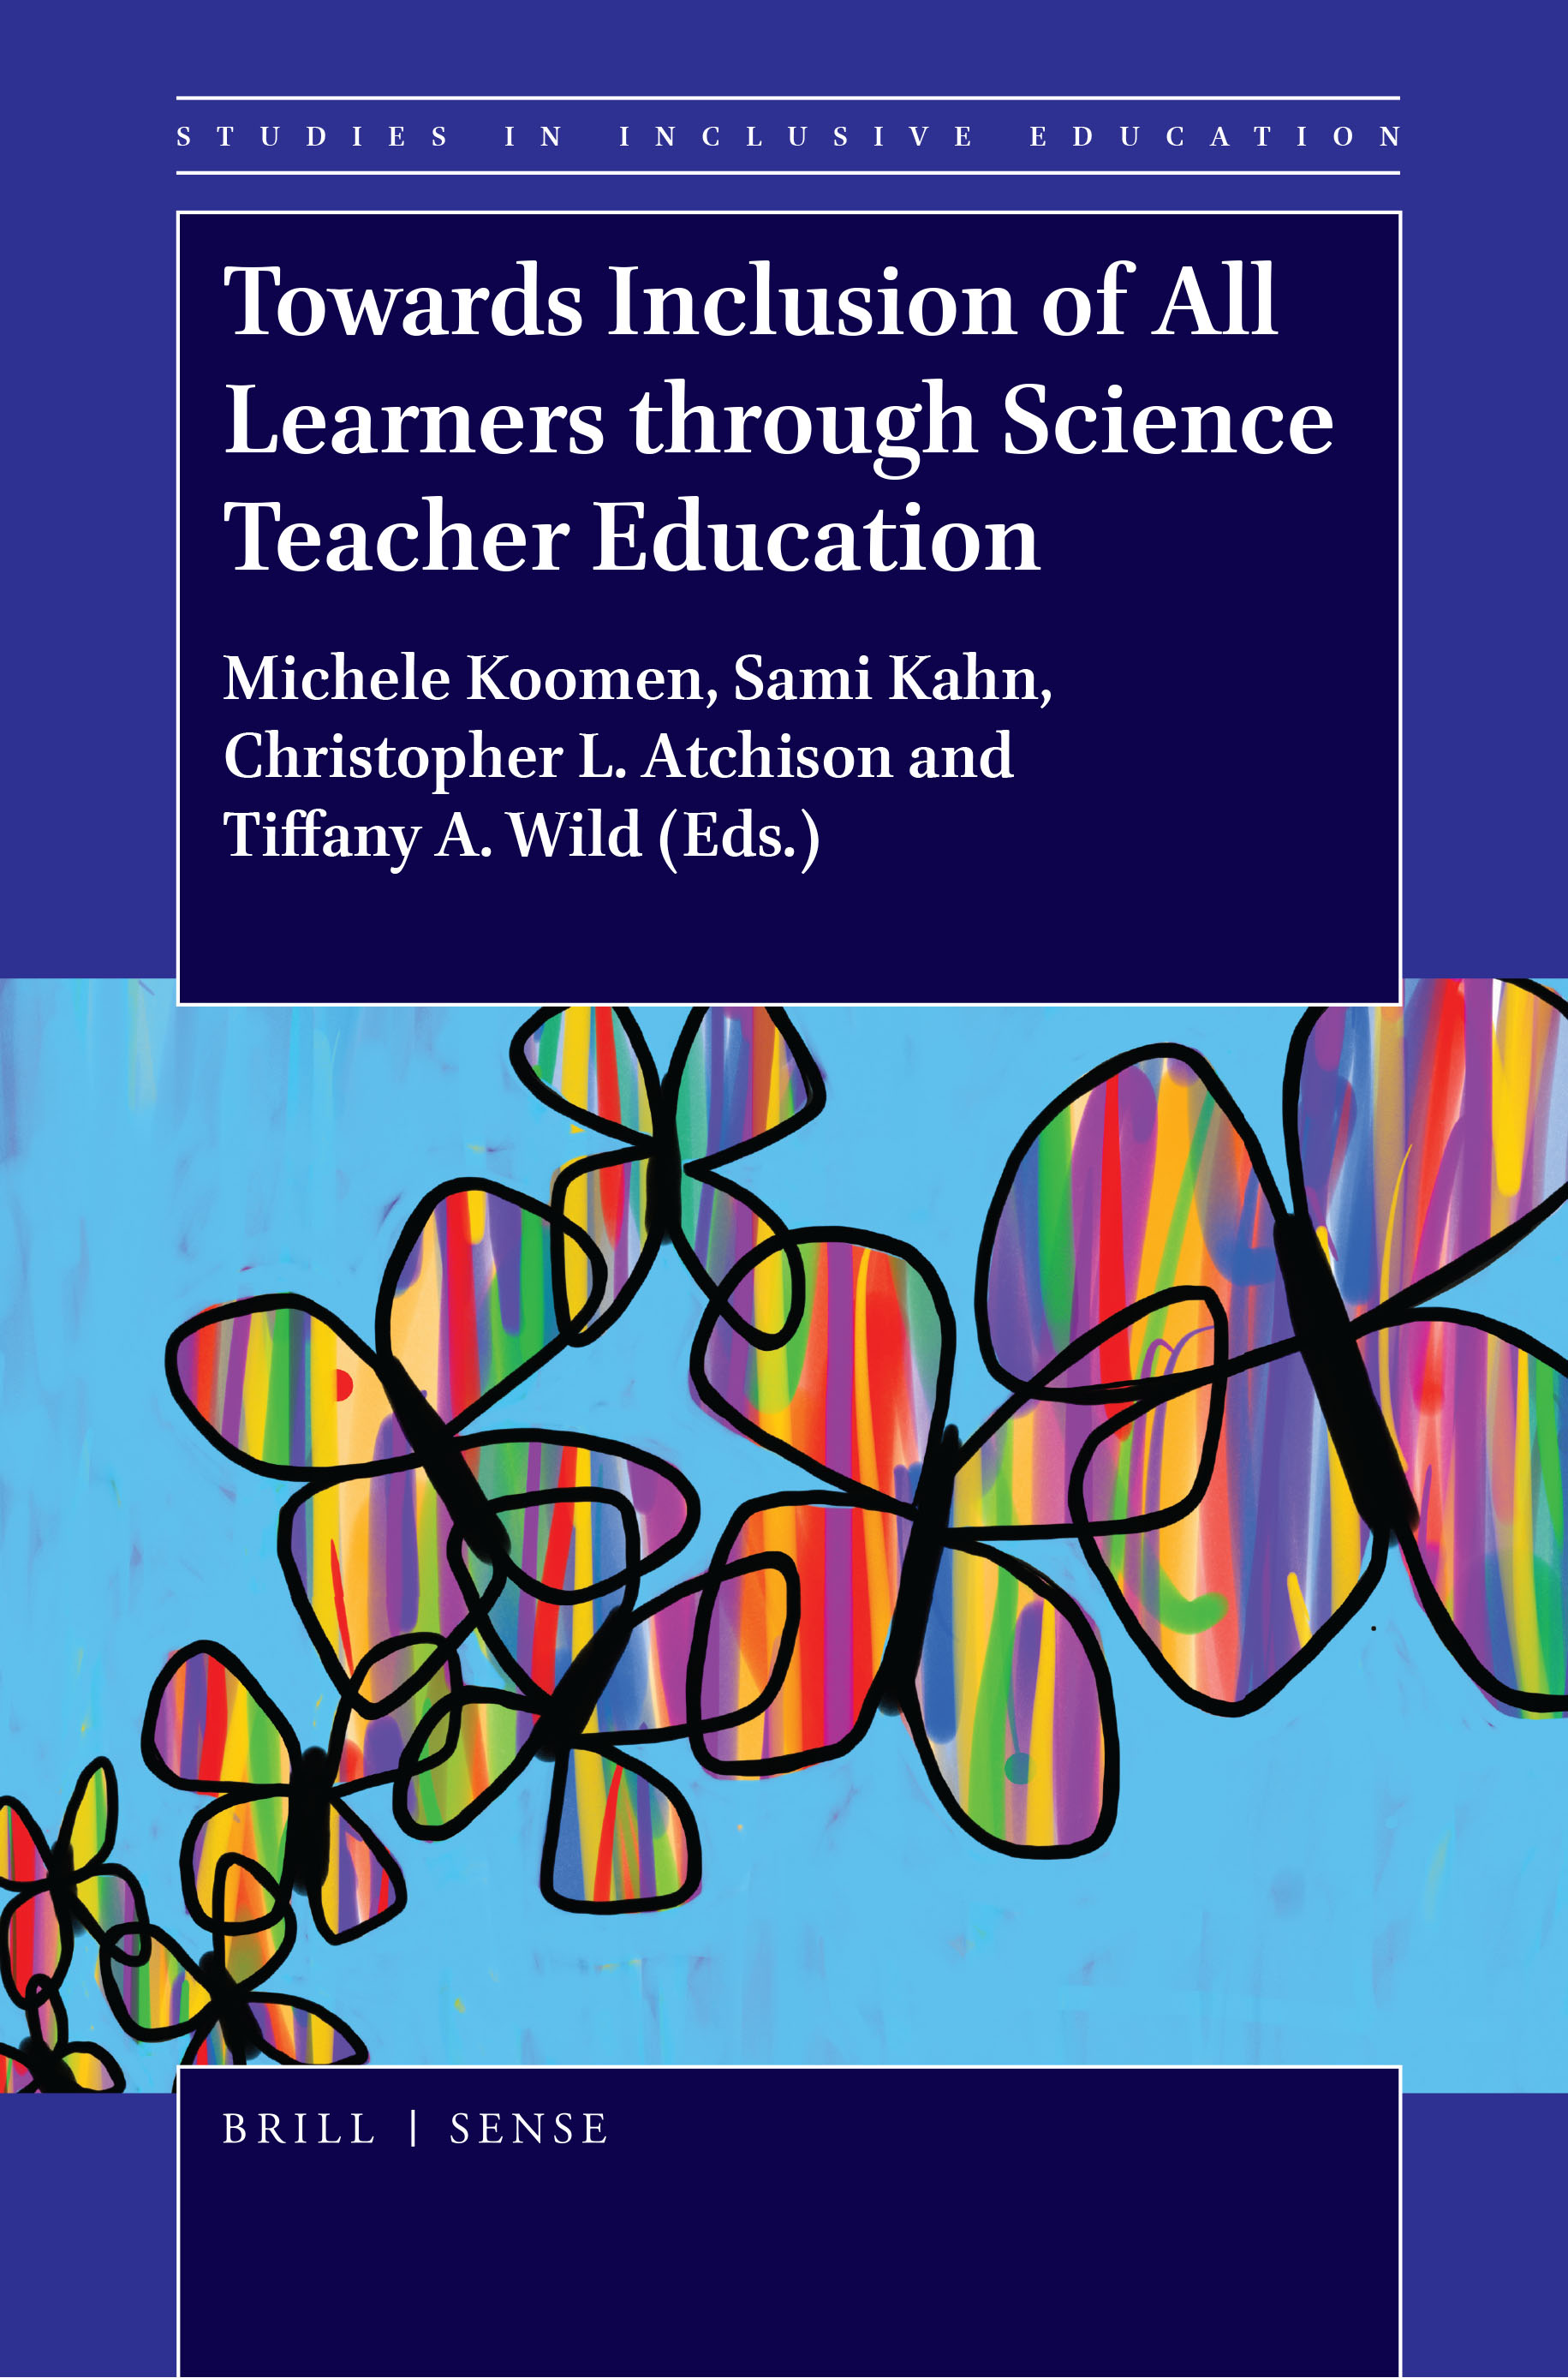
\includegraphics[width=0.7\linewidth]{fig1.jpg}
\end{figure*}
\end{@twocolumnfalse}
%% AUTHOR INFORMATION

\pagebreak
\clearpage
\begin{large}
It is a pleasure to receive an invitation to submit a review for the book titled \textit{Towards Inclusion of All Learners through Science Teacher Education}. The contributors include four well-known leaders in inclusive science education complemented by a spectrum of authors American and international, in pre-service and graduate science education, pre-service and graduate special education, science research, special education practitioners, classroom teachers, graduate students, and students through case studies and interviews.

The book presents an excellent overview of current practices in schools, descriptions of individual and team efforts to improve practice, and emerging innovations such as the application of Universal Design for Learning (UDL) and Assistive Technology (AT) as promising possibilities if we are to provide equitable science for students with disabilities.  Stories from students; descriptions from practitioners in K-12 education; strategies and experiences from post-secondary methods instructors in science education and special education are interspersed throughout the book.  Strategies applying the principles of UDL and scaffolding are shared. Section three contains several highly innovate efforts in practice.

Literacy specific to science is addressed.  The authors note that all students need to develop competency in receptive and expressive communication specific to science.  Suggestions are offered on how to support students in learning vocabulary, organization, speaking and writing.  Assessment is noted as a major challenge, particularly within the frameworks of accountability testing spearheaded by the United States Department of Education and individual state departments of education which are often incongruent with inquiry and higher order reasoning abilities stressed in a rigorous STEM curriculum.  Section 7 points out the need for teacher advocacy, peer support, communication with role models and peers, mentorships and internships as important and valuable to students with disabilities.  Physical and sensory disabilities are low incidence and distributed across the general population so particular efforts are needed by teachers to access resources and opportunities.

\subsection*{Summary}

The introduction of this book provides a sound foundation for all teachers relating to their professional responsibilities as an educator.  It describes the shortcomings of current practice regarding equitable science learning opportunities for student with disabilities.  It notes that practicing teachers support the need for additional training in teaching students with disabilities.  The book contains stories from students and practitioners that describe shortcomings and suggestions for improving teacher preparation. They note the need for Disability Studies in Education specific to the content areas being taught, particularly in all STEM fields.  Much of the learning in STEM is built on previous concepts and skills making gaps in learning cumulative, becoming overwhelming at the secondary school and/or postsecondary level, depriving the student an opportunity to pursue a career in a STEM field.

The first chapter provides insights regarding low expectations and soft inclusion where students with visual impairments are marginalized and ignored.  The authors note the value of prior exposure, accessible materials, and adequate time to engage in the full educational experience with accommodations when possible. The stories illustrate that students are very conscious of other students and every effort must be made to include them in as normal of a context as possible. They note the many advantages of utilizing new technology and the need for teachers to be a part of the search for accessible opportunities that enable equitable opportunities to engage and learn.

Chapter 2 highlights challenges faced by deaf and hard of hearing students by providing insights relating to the dearth of deaf individuals in STEM fields.  The authors describe classroom science teachers as lacking even a basic understanding of what it is like to be a deaf learner in a science classroom.  The fact that it is impossible to simultaneously observe an experiment and focus on the interpreter is generally lost. The authors point out that the interpreters often lack core science knowledge and are unable to adequately share the concepts being taught because they do not understand what the teacher is teaching.  They also point out that much of the vocabulary in secondary school science is new and unfamiliar to the learner.  The recommendations at the end of the chapter are excellent, but probably insufficient.  Even in schools for the deaf it is unlikely that a student will receive equivalent education in the sciences because of the absence of teachers with in-depth content knowledge and a thorough awareness of the learning needs of a deaf learner.  The authors note the need for role models and communication.  Technology provides some hope in that through the Internet it is possible to connect  with peers and practicing scientists with disabilities, but only if teachers make the effort to become informed and facilitate these linkages.  

Chapter 3 describes challenges faced by students with dyslexia and the need for allies, mentors and advocates for all students with disabilities.  The chapters illustrate the limitations of teacher preparation programs and the utilitarian nature of teaching in general. There is a tendency to focus on general practices that relate to large numbers of students with diminished emphasis on low incidence disabilities.  As a consequence only the most brilliant are able to navigate a successful career in a STEM discipline.

Chapter 4 describes the importance of appreciating the learner and taking the time to become familiar with the unique learning needs of each student.  It illustrates that teachers that are remembered are those who make learners feel important and appreciated.  They are aware of the needs of students regarding student socialization and don’t engage in behaviors that demean a learner who makes errors or performs poorly. Effective teachers create a warm environment that promotes learning. This same aspect was emphasized by the author of Chapter 5 relaying the experiences of students with Autism Spectrum Disorder.  Chapter 6 contains stories from students with diagnosed intellectual disabilities and emphasizes the importance of being a good listener, providing hands-on experiences and showing enthusiasm as important teacher qualities.

The summary in Chapter 7 provides an excellent synthesis of the suggestions offered in the first 6 chapters.  The guidelines provide practicing teachers with a series of suggestions for reflection and directions on how to improve professional practice for all students.  In itself it is a concise summary of best practice.

Section 2 begins with a definition of inclusive science learning as a critical element in providing equivalent educational opportunities for students with disabilities.  This is especially important in the sciences where more advanced concepts build on prior exposure to core knowledge built during earlier years of schooling.  If students are not exposed to these concepts because of pull out programs or segregated classrooms using some form of tracking, students with disabilities miss this critical exposure. They suggest an approach labeled as dramatic inquiry where students can be positioned to explore science as a shared task with peers and teacher guidance.

The following chapter describes the application of universal design is a valuable mechanism in science teaching as a means to mediate the effects of limited language and literacy skills.  The authors note challenges with vocabulary and text comprehension. They suggest that the application of UDL and AT as valuable applications for reducing barriers to learning.  In the chapter language barriers and possible solutions are presented.

Sami Kahn does an outstanding job of describing how a deficit model by its very nature makes science “exclusionary” for the vast majority of students with disabilities.  In Chapter 10, she presents strength based frameworks as a means of building on students strengths to provide a positive environment where students can thrive. She shares real experiences where students have excelled through using strength-based instructional practices.  She notes the importance of teachers making an active effort to identify student interests and strengths through multiple means, one being through conversations with the students themselves, and activating these areas in the science classroom.  She notes that providing students with “choices” can have a profound effect on classroom atmosphere.

Technology can be a valuable tool in any educational context when teachers make an effort to seek out alternative resources.  A multitude of devices exist that can provide access in means that were not possible a short time ago. Students with physical and/or sensory deficits can access information, resources, alternative inputs, and utilize physical aids to do experiments and provide physical models.  The utilization of Universal Design, the design of products and environments to be usable by all people, to the greatest extent possible, without the need for adaptation or specialized design,” can place educators at the forefront of a more equitable world.   In Chapter 11, Sheryl Burgstahler describes how she has applied Universal Design in the development of an on-line learning environment followed by numerous suggestions.

UDL has evolved as a natural follow-up to the success of Universal Design in architecture which has made life in the United States accessible to vast numbers of individuals with physical and sensory disabilities.  UDL is a proactive approach that scaffolds and supports the curriculum process to meet the needs of all learners and minimize the need for individual accommodations and modifications.  It is noteworthy that UDL focuses on curriculum design not learner needs.  The need to understand the learning needs of individual students is still the most important factor in becoming an effective teacher.  Chapter 12 presents suggestions that can provide students with multiple means of action and expression where students can share what they have learned and are able to do.

Section 3 provide s examples of how teachers  have implemented instructional practices that enable all students to acquire core disciplinary ideas and science content knowledge through inclusive strategies and the application of UDL.  In Chapter 13 the author describes an approach to physics where an assortment of learning centers with the addition of tactile models are set up in his office. They provide opportunities to explore the concepts independently to enrich the learning experience.  He states that he has found the approach not only good for students with visual impairments but equally good for other students as well.  The approach has several advantages: 1) It provides additional time outside of class to gain essential concepts which in general is very important for students with disabilities 2) It provides an additional tactile element, an essential accommodation for students with visual impairments but good for students in general 3) It presents opportunities for working in small groups for students who would benefit. 

Chapter 14 presents a crosscutting strategy applying the principles of the UDL Framework.  The authors share a nice strategy to help students’ better see relationships across core concepts.  The principle of scaffolding is shared which is very important for students with disabilities because ineffective teachers often leave gaps which require that an alert teacher build the core knowledge essential for grasping the concept in the lesson.   The authors apply a strategy in Vignette number one, and Vignettes two \& three describe the teacher and student responses.  

In Chapter 15 the authors describe a five year process in which an instructional unit on Frog Calls was implemented utilizing two deaf students as participants in field research.  There were modifications in working with ASL interpreters and the application of sonograms which provided tactile illustrations of the frog sounds.  In addition, they worked on collaborative activities during the field work that enabled the deaf students to be active participants in all aspects of the field research.  The results were exemplary.  The chapter illustrates that changes are not always easy and short term.  If we are to transform education to make learning accessible for all students, developing an effective teaching model takes time and requires considerable refinement. Again the authors noted that the modifications that were employed benefitted not only the deaf students but many other students as well, reflected in an overall post-test mean gain score of 11.6\%.

Chapter 16 addresses engineering, a discipline with relatively severe underrepresentation for persons with disabilities, women, and minorities.  The introduction  of engineering design allows students to search for solutions to real problems an element which is generally lacking In the traditional curriculum.  The chapter describes a case study which illustrated the improved understanding of three disciplinary core ideas (DCI) of engineering. Chapter  17 describes a program where students with intellectual and developmental disabilities are integrated in a pre-service course for special education and science students. A cooperative group instructional approach is used and the 5E learning cycle served as the mechanism for content organization.  The course included the development of a collaborative communication model that engaged all students in the group.  Groups were 3-5 students with all groups having at least one student with a disability.  All students were participants in the evaluation process.  They employed pictures, presentations, reciprocal questioning, and probing for deep and more extensive responses. In the concluding comments the students describe how they built community in a diverse group with a deeper understanding of how to work as a team along with improved science content knowledge.

The chapters contained in Section 3 present several highly innovative approaches to inclusive education outside of the parameters most educators think.  If education is to be inclusive, tinkering with our current approaches is not likely to result in a major transformation.  The approaches shared in Section 3 include examples that are “outside the box” which can act as a stimulus for innovative thinking.

Section 4 is an effort to transition into practical strategies in promoting inclusive science education.  In Chapter 18 the authors provide an excellent summary of two critical elements, scaffolding and UDL. They address two major principles: 1) Scaffolding requires a relationship between the student and teacher in determining and supporting learning tasks in which the student can engage and grow, and 2) UDL provides multiple means of engagement, representation, and expression which provides the student some flexibility to show what they have learned and what they are able to do.  This goes a long way toward meeting the goals of inclusive education.  My only caution is that every human being is unique and any individual student may require unique adaptations in order to maximize engagement in the learning process. The authors use sink and floating activities in describing how one can apply the strategies.

Higher order thinking is a challenge for all educators and critical for reasoning in science. Developing comprehension and inquiry skills is very important. The authors in Chapter 19 present steps in moving from a traditional classroom to one which is inquiry based. They stress that good science teaching involves exploration and science investigations using hands-on resources.  Doing science is the focus of Chapter 20.  Students need to collect evidence and developing explanations based on empirical data. They need to engage with others and engage in negotiation when engaging in argumentation. Students need to undergo multiple drafts with improved refinement. The authors present a Four Corners strategy in order to ground the concept with a real world application.

Section 6 has a focus on developing science literacy.  Successes in all aspects of life include proficiency in communication through both receptive and expressive channels.  Reading and writing are fundamental skills which must be reinforced in all aspects of the instructional process. Vignettes are shared to illustrate the strategy. The authors in Chapter 21, using density as a basic science concept, start by doing science, sharing experiences, utilizing science notebooks, applying concept oriented reading instruction (CORI), and fostering the academic language of science in the learning process. Chapter 22 has an emphasis on science literacy. In it,  Michele Koomen states that developing habits of mind requires knowledge and application specific to the discipline being studied. Students need to read, write, think and communicate in science: read aloud, shared reading, applying graphic organizers, questioning the author and summarizing are all essential skills for science literacy.  The author shares the application of several tools to support students with vocabulary, organization, writing, argumentation, and explanation.

Section 7 brings to light challenges contained in science assessment.  The immense quantity of core knowledge in the broad fields of science and social studies presents unique challenges in assessment.  This is compounded by difficulty in assessing higher order reasoning and measuring student understanding of core concepts across all of the disciplines.   Chapter 23 exposes the reader to a variety of measurement tools noting both their purpose and limitations.  The authors briefly share some of the accommodations currently being applied for students with specific types of disability.  Chapter 24 notes that in order to address the goal of scientific literacy as noted in the Next Generation Science Standards (NGSS) we must investigate the understandings of Science Inquiry (SI)  and Nature of Science (NOS).  An oral assessment tool, Young Children’s Views About Science (YCVS) is described along with scoring and research findings from the results of the assessment. It is an excellent summation about the limitations of current assessments, particularly in the underassessment of science knowledge and understanding of science by students with disabilities.  The authors bring to light the tremendous challenge of assessment in education for all students, with even greater challenges for those possessing any and all characteristics of diversity.

In Chapter 25 case studies of four individuals with visual impairments are summarized containing elements that attributed to their success in STEM fields. Emphasis is on the importance of role models, peer support, teacher advocacy, mentorships, and internship opportunities. In Chapter 26 the author notes the compounding impacts of additional factors affecting participation by persons with disabilities in STEM fields.

The chapter focus is on three elements: disability, race, and urban education.  Gender should be cited as well.  There is no question that social persuasions, unsupportive messages from teachers, low expectations, limited efforts toward accommodation, and limited opportunities to engage in rigorous science learning activities all play a part in impacting performance by students with disabilities in STEM fields.

Section 8 draws on experiences of practicing teacher educators who share successful strategies in their own teaching. In Chapter 27 the authors, Teresa Shume and Keri Desutter, share the preparation process and implementation of a lesson based on collaboration and co-teaching between a science educator and special education professor.  The description is excellent and is a model that can be employed in almost any pre-service program for educators.  Unfortunately it appears that the collaboration is only on one lesson and does not appear to capitalize on the associated student field experiences in the program. It is a good start that needs more comprehensive implementation if the professors wish to model a comprehensive program reflecting inclusive practice. 

Chapter 28 presents stories from teachers with disabilities.  The authors share experiences from England, which appears to have similar legislative mandates regarding accessibility to those in the United States.  They emphasize pre-planning and preparation so the teaching platforms are accessible and teacher mobility is addressed.  They note that during the instructional process students adapt well to accommodations and limitations relating to having a teacher with a physical disability.  It is important for all students to see persons with disabilities in classroom as teachers.  I was pleased but not surprised with the comment, “from pupils I have been treated as normal without exception from day one.”  The authors of Chapter 29 point out that it is difficult to determine the degree to which inclusion is practiced in general education classrooms, both in terms of time students spend in the regular classroom and the degree to which the curriculum is adapted to best fit their learning needs.  They discuss revisions in a teacher preparation program using UDL and Understanding by Design (UbD) to develop units of instruction and strategies for designing modifications and adaptations for students with disabilities. The approach describes a collaborative process which includes pre-service teachers, pupils, classroom teachers, and students. 

Chapter 30 provides a wonderful description of the need for flexibility in a utilitarian culture.  It is a story of a bright young man with a severe physical disability who completed a pre-service teaching program in Earth Science.   The author noted examples of some of the challenges faced during student teaching.  What was missing was a willingness to adjust the student teaching situation to the student.  Major challenges for almost all persons with disabilities are time constraints. Personal hygiene is an essential factor in functioning in our social system and work environment, as is adequate rest.  From the description shared in the story, it appeared that the university was unwilling to make adjustments such as reducing the number of classes the student teacher needed to teach each day. That factor alone created an untenable situation in the context of providing a successful and rewarding experience for a well deserving student.  The world desperately needs role models, one being teachers with disabilities in our classrooms.  Supervisors and colleagues must make adjustments so individuals who have the capabilities and interest can function well in the classroom.  I closed this chapter with considerable sadness, the likely loss of a stellar individual who had so much to contribute to the teaching profession and society in general, by an inflexible adult culture unwilling to make appropriate accommodations.

The final chapter is an excellent summation of the contributions of the authors.  It contains a wealth of ideas for reflection for improving one’s own teaching and directions for educational reform.  An area in which the book fails and society fails in general, is an inability to demonstrate flexibility in order to accommodate the success of others. There is simplicity in life; every individual needs to feel important and appreciated, some more often than others.  It is a responsibility of society to provide circumstances where every individual, when he/she gives full effort, can experience success.  This relates to childhood, schooling, careers and social endeavors.  The focus must be on the individual, what he/she is capable of learning and what he/she can do.  Secondly, when someone performs well it must be acknowledged and supported. The application of UDL to life is the key to a better world. Individuals need multiple means of engagement, representation, action, and expression.  Individuals need opportunities to make choices. A sense of success breeds persistence and persistence is a key to success.  Our focus must always be on the individual.

Advances in technology have greatly increased access to resources and devices that allow for greater participation by all students in educational endeavors.  However the essence of a quality educational experience relies greatly on the teacher-student relationship and the capacity/willingness of the teacher to provide the student with learning opportunities that enable success with reasonable effort on the part of the student. My perceptions are at the class room level, although there is much greater awareness of students with disabilities, many students are not receiving learning experiences in science that enable them to be fully engaged.  The impact of passive participation, along with lower expectations, is often cumulative. The consequences are obvious when one looks at the underrepresentation of persons with disabilities in STEM fields. This book illuminates many factors that exist in present practice, which must be resolved if students with disabilities are to ever receive an equivalent and equitable science education.

This book brings to light many of the major issues confronting inclusive science.  It is a methods book that can be used as the primary textbook in both science methods and special education methods. It is well suited for graduate classes in curriculum development and instructional strategies.  It is an outstanding resource for graduate seminars relating to educational equity and educational reform. I see it as an excellent inschool resource which can be used in in-service training and professional development. I see it as a reflective resource well suited for the personal library of any teacher, curriculum specialist, or administrator.

\subsection*{Personal Statement}

Dr. Greg Stefanich was involved in some aspect of science education regarding students with disabilities in science for 63 years.  His initial experience with disability followed a personal affliction with polio at the age of 12. Polio yielded: a significant loss of coordination; reduced strength; the need for considerably more rest than peers; school absenteeism while receiving physical therapy; challenges with weight (i.e. six feet tall and 118 pounds as a high school sophomore); and social challenges through puberty and adolescence. After graduating from high school in 1961, he completed his Bachelor of Science Degree in 1965 with majors in Chemistry and General Science, an MA in Science Education in 1968, and a doctorate in Curriculum and Supervision in 1971.  He spent four years as a secondary school science teacher and 45 years in postsecondary education, primarily as a science education professor.  He has been deeply committed in efforts to improve the educational experiences of students with disabilities in science throughout his adult life.

\end{large}
\clearpage
\section*{REFERENCES}\par 

\leftskip 0.25in
\parindent -0.25in 
Koomen, M.L., Kahn, S., Atchison, C.L.,\& Wild, T.A. (Eds.). (2018). Towards inclusion of all learners through science teacher education. Leiden, The Netherlands: Brill/Sense

Available at:
\url{http://brill.com/view/title/38174}
\end{document}